\subsection{Client}

    \subsubsection{Spielansicht für einen Spieler}

    \begin{figure}[H]
        \centering
        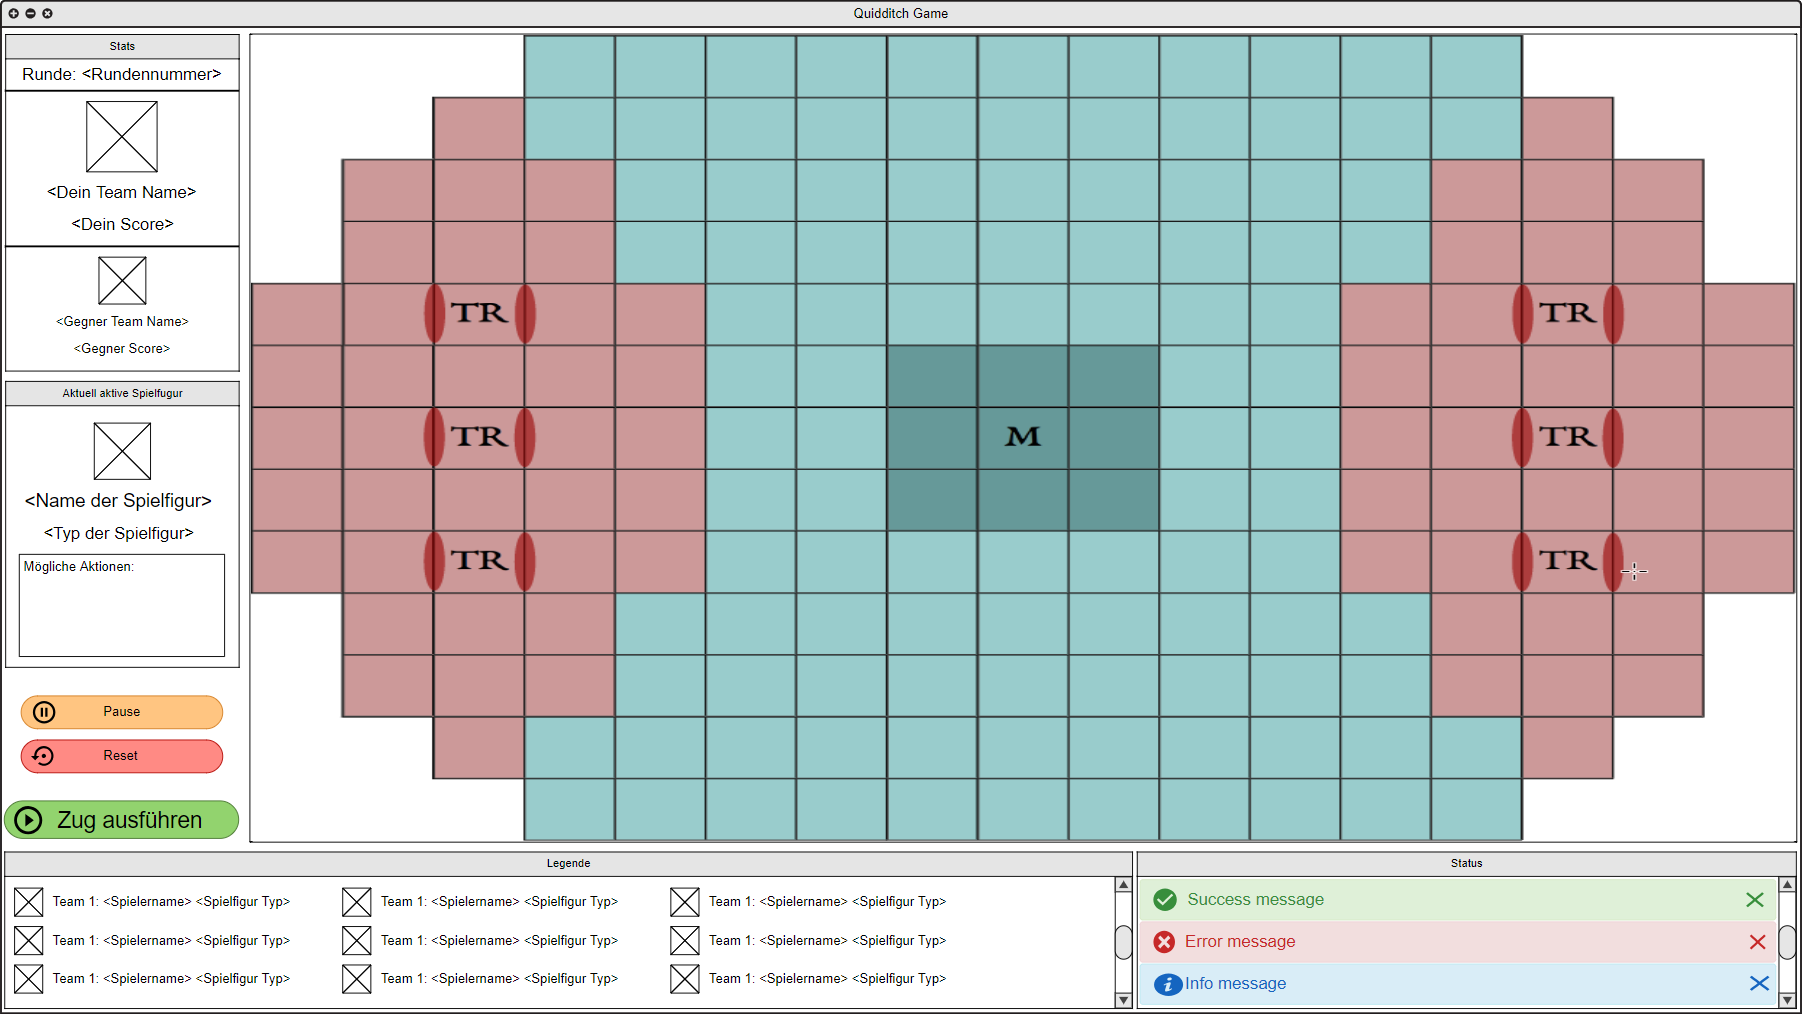
\includegraphics[width=\textwidth]{images/InGamePlayer.PNG}
    \end{figure}

    In der Spielansicht kann ein Spieler das aktuelle Spielgeschehen verfolgen und sein Züge ausführen. Dabei ist die Oberfläche in mehrere Teile unterteilt.\\
    Im \textit{Stats} Bereich werden grundlegende Informationen über die aktuelle Partie und die beiden Teams dargestellt. Das Team welches an oberster Position steht ist momentan am Zug. Der darunter liegende Bereich ist der \textit{Fan} Bereich. Hier kann der Spieler auswählen ob und welcher Fan seine Aktion ausführen soll. Darunter befinden sich drei Buttons mit dem entweder das Spiel \textit{pausiert} werden kann, alle Veränderungen die man in der aktuellen Runde getätigt hat \textit{zurücksetzen} kann oder seinen Zug endgültig \textit{ausführen} kann. Am unteren Rand der Oberfläche ist eine \textit{Legende} mit einer Übersicht über alle Spielfiguren des eigenen und des gegnerischen Teams zu sehen. Daneben befindet sich ein Feld in dem Statusmeldungen angezeigt werden können. Beispiele für solche Statusmeldungen sind z.B. eine Benachrichtigung über ein Faul oder über das erfolgreiche Ausführen eines Spielzuges. Der größte Teil der Oberfläche nimmt dass eigentliche Spielfeld ein. Hier werden alle Spielfiguren in den Feldern angezeigt auf denen sie sich gerade befinden. Ist man am Zug und klickt auf einen Spieler, so werden alle Züge, die von der Spielfigur ausgeführt werden können farblich hervor gehoben. Der Spieler kann diese Aktionen dann durch weitere Klicks ausführen und die Prozedur gegebenenfalls für weitere Spielfiguren wiederholen. Ist man nicht am Zug so werden alle Eingabemöglichkeiten, mit Ausnahme des \textit{Pause} Buttons deaktiviert.
    

    \subsubsection{Spielansicht für einen Beobachter}
        
    \begin{figure}[H]
        \centering
        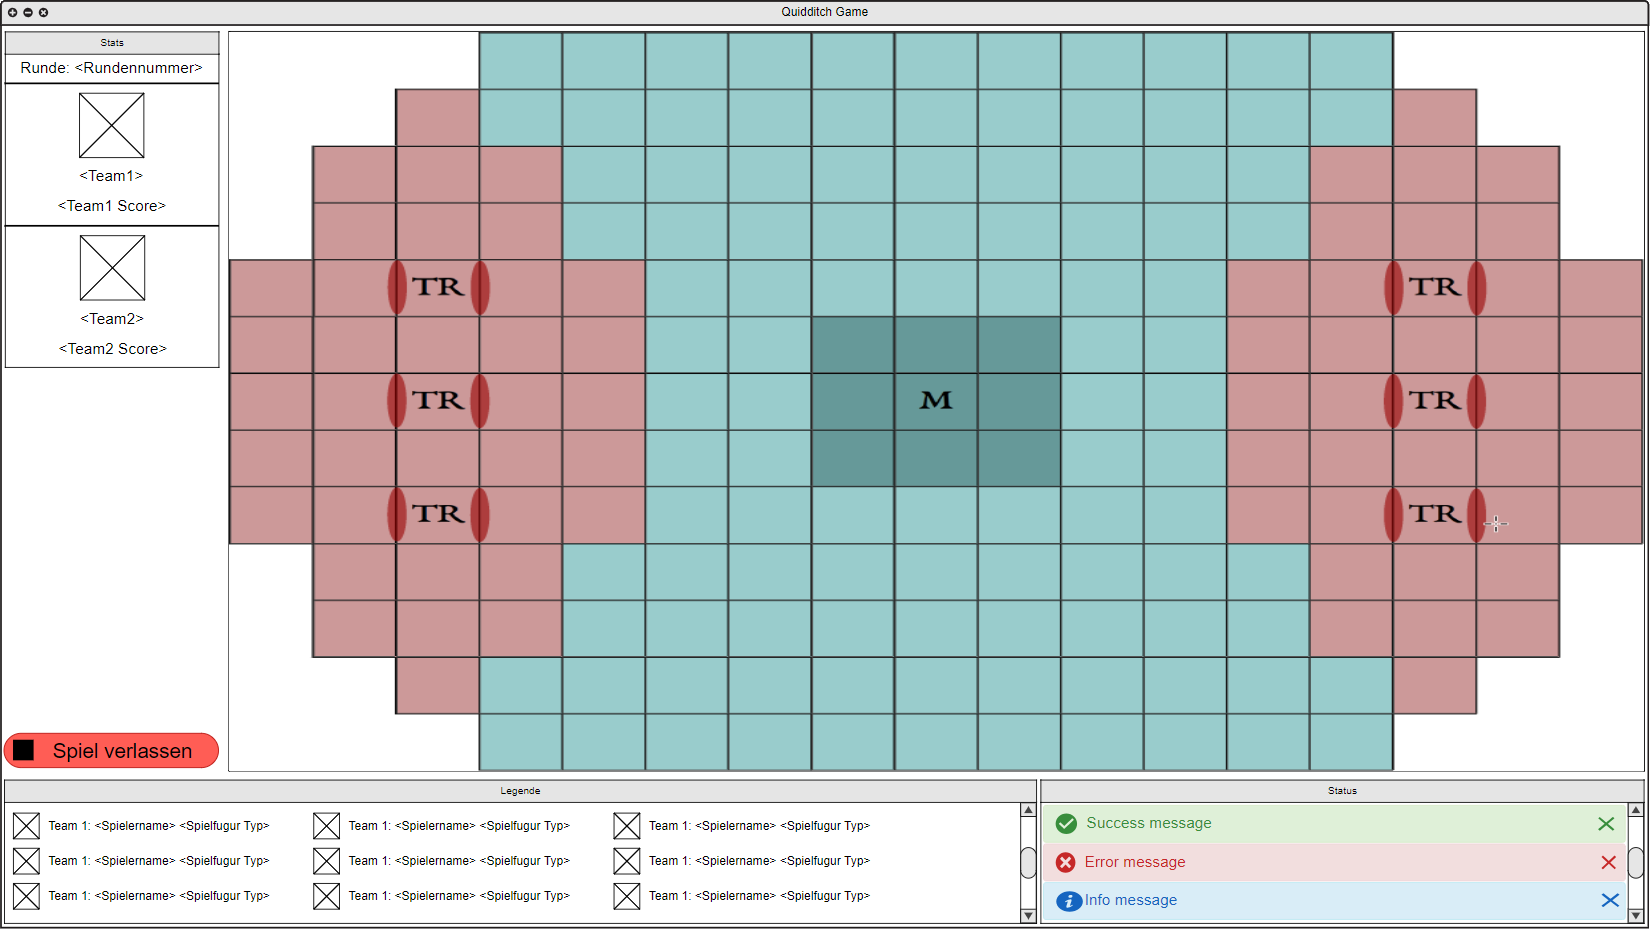
\includegraphics[width=\textwidth]{images/InGameObserver.PNG}
    \end{figure}

    In der Spielansicht kann ein Beobachter eine Partie wischen zwei anderen Gegnern passiv verfolgen. Die Oberfläche ist im wesentlichen gleich aufgebaut wie die Oberfläche, die die Spieler sehen. Jedoch sind beim Beobachter alle Felder die zur Eingabe dienen deaktiviert und teilweise ausgeblendet. Die einzige Interaktion, welche durch einen Button ermöglicht wird ist das vorzeitige \textit{verlassen} einer Partie.